\section{Grundlagen}
Die folgenden zwei Abschnitte definieren die \ac{ki} und Chatbots. Sowie die drei Ethiker die untersucht werden. 

\subsection{Künstliche Intelligenz}
Dieser Abschnitt definiert die Bedeutung der \ac{ki} aus Sicht der Autoren. Bereits viele Menschen haben sich daran versucht den Begriff der \ac{ki} zu definieren. Leider gibt es bislang keine allgemein anerkannte und eindeutige Definition. Bereits bei der Frage \enquote{Was ist Intelligenz} gibt es nicht eine einzig wahre Aussage\footnote{vgl. \cite{Intelligenz}}. Sicher ist, die Menschen nehmen eine besondere Stellung unter den Lebewesen ein. Diese besondere Stellung basiert unter anderem auf unserer Intelligenz. 

Der \ac{ki} Pionier John McCarthy veröffentlichte bereits 1955 eine Exposé in der McCarthy auf die Künstliche Intelligenz eingeht. Die Exposé definiert die \ac{ki} wie folgt,
\begin{quote}
		\glqq For the present purpose the artificial intelligence problem is taken to be that of making a machine behave in ways that would be called intelligent if a human were so behaving\grqq.\footnote{\cite{PROPOSALMcCarthy}}
\end{quote}
Diese Definition ist allerdings zu vage. Denn für viele Menschen gilt ein Roboter, der einem Hinderniss ausweicht schon als intelligent. Für Informatiker ist das Ausweichen eine logische Schlussfolgerung aus eingehenden Sensorsignalen. Bekommt der Roboter die Sensoreingabe, dass er vor einem Hindernis steht, so ändert dieser aufgrund der Programmierung die Richtung.

Einen weiteren Versuch die \ac{ki} zu definieren, unternahm Elanie Rich bereits 1983,
\begin{quote}
	 \glqq Artificial Intelligence is the study of how to make computers do things at which, at the moment, people are better\grqq.\footnote{\cite{ArtificialIntelligence}}
\end{quote}

Das nächste Beispiel nennt eine \glqq Sache\grqq\ in der Computer uns überlegen sind. Computer sind uns im Speichern von Daten und der Berechnung von nummerischen Aufgaben überlegen. \newline
Dagegen sind die Menschen in der Erkennung von Objekten den aktuellen Algorithmen überlegen. Sobald wir einen Raum betreten findet im unserem Unterbewusstsein eine Objekterkennung statt. Wir erkennen sofort, dass der Raum beispielsweise drei Fenster, zwei Türen und vier Wände hat. Gleichzeit erkennen wir Gegenstände im Raum, wie Tische, Stühle und Bildschirme auf den Tischen. Danach schließen wir darauf, dass dieser Raum ein Computerraum sein muss. Dieser Entschluss wird gefasst mit Hilfe von Wissen was wir bereits haben und Erfahrungen die wir erlebt haben. Wir verknüpfen innerhalb von Sekunden die Objekte und unser vorhandenes Wissen, um einen Entschluss zu fassen. \newline 
Die aktuelle \ac{ki} steckt hier noch in den Anfängen. Moderne Algorithmen können zwar mehr oder weniger gut Objekte erkennen und diese Greifen, aber die \ac{ki} hat kein Gesamtbild der Umgebung. Die zwei Beispiele sollen zeigen, dass es Dinge gibt die ein Computer aktuell besser kann aber auch Dinge die ein Computer noch nicht besser kann als ein Mensch. 

Die KI ist ständig im Wandel. Gilt ein Problem als gelöst dann verschieben sich die Aufgabenbereiche der KI.   
Wie sich die Aufgabenbereiche der \ac{ki} verändern zeigen zwei Beispiele. Im Jahr 1997 schlägt IBM's Deep Blue den Schach Weltmeister Garri Kasparow\footnote{vgl. \cite{SchachQuelle}}. Dies hatte zur Folge, dass die \ac{ki}-Forschung nach und nach das Interesse an Schach verlor. Aus ihrer Sicht gilt Schach heute als gelöst. \newline
Anfang 2016 gab es einen weitere Sensation. Die \ac{ki} Alpha Go von Google schlägt einen menschlichen Go-Profi\footnote{vgl. \cite{GoQuelle}}. Auch diese Entwicklung führt dazu, dass sich die \ac{ki}-Forschung auf neue Aufgabenbereiche konzentrieren wird. 

Es gibt noch zahlreiche Gebiete in denen wir Menschen der \ac{ki} weit überlegen sind. Durch die rasante Entwicklung der letzten Jahre in der \ac{ki} werden immer mehr Anwendungen und Produkte mit ihr verknüpft. So setzen Firmen bereits sogenannte Chatbots, mit einer \ac{ki} im Hintergrund, zur Kundenkommunikation ein.

\subsection{Chatbot}
Ein Chatbot ist eine Art Maschine für die Kommunikation mit dem Menschen. Meistens besitzt ein Chatbot ein Dialogsystem. Das heißt der Kommunikationspartner kann per Texteingaben mit dem Chatbot kommunizieren. Der Mensch stellt eine Frage per Texteingabe. Der Chatbot versucht daraufhin die Frage zu interpretieren und generiert eine Antwort.

Die Idee eine Maschine zur Kommunikation mit dem Menschen einzusetzen ist nicht neu. Bereits 1966 entwickelte Joseph Weizenbaum ein Computerprogramm, dass die Kommunikation mit Mensch und Computer ermöglichte. Das Programm wird \glqq ELIZA\grqq\ genannt. Im Hintergrund verwendet das Programm ein sogenanntes \glqq Pattern Matching\grqq\, was einer Mustererkennung entspricht. Mit dieser eigentlich einfachen Technik, war es möglich den ersten Chatbot zu programmieren. Eine einfache Version von ELIZA verwendet einen Theasaurs. Dies ist eine Art Wörterbuch, dessen Wörter durch Relationen miteinander verbunden sind. So ist zum Beispiel Mutter mit dem Wort Familie verbunden. Des Weiteren gibt es ein vordefiniertes Set von Phrasen. Diese Phrasen sind häufig Fragen oder Aufforderungen. Ein Beispiel ist auf der deutschen Wikipedia-Seite zu finden. 
\begin{quote}
    Benutzer: Ich habe ein Problem mit meinem Vater.\newline
    ELIZA: Erzählen Sie mir mehr über Ihre Familie! 
\end{quote}
Hier sieht man wie das Wort \glqq Vater\grqq\ mit dem Wort \glqq Familie\grqq\ in einer Relations steht. ELIZA verwendet dann eine passende Phrase zum Wort \glqq Familie\grqq.
\begin{quote}    
    Benutzer: Krieg ist der Vater aller Dinge.\newline
    ELIZA: Erzählen Sie mir mehr über Ihre Familie!
\end{quote}    
Im zweiten Beispiel verwendet ELIZA die gleiche Phrase wie im ersten Beispiel. An dieser Stelle kann man sehr gut sehen, dass ELIZA die Bedeutung des Satzes in keiner Weise versteht. Es wird rein nach \glqq Pattern Matching\grqq\ vorgegangen. Es wird eine passende Phrase zu einem passendem Pattern gesucht.\footnote{vgl. \cite{WikiELIZADE} und \cite{WikiELIZA}}    

Heute setzen immer mehr Firmen Chatbots in der Kundenkommunikation ein, speziell beim Support von Kunden. So greifen Firmen wie Lufthansa, Zalando, Opel, etc. bereits auf Chatbots zurück. Die Chatbots sind zwar noch nicht voll integriert, aber erste Experimente finden bereits statt.\footnote{vgl. \cite{UnternehmenChatbots}} \newline
Lufthansa startete im November 2016 den Chatbot \glqq Mildred\grqq. Dieser Chatbot ermöglicht die Suche nach dem günstigsten Preis für einen Flug. Die angebotenen Flüge liegen alle innerhalb der kommenden neun Monate. Der Chatbot ist in den Facebook-Messenger integriert. Für eine Suche geben die Nutzer Abflug- und Zielflughafen an. Auch die internationalen Buchstabencodes können verwendet werden. Der Chatbot erkennt auch die Buchungsklassen der Lufthansa. Über die mobile Version von LH.com kann dann das angebotene Ticket gebucht werden. Erste Tests des Chatbots zeigten bereits Schwächen des Chatbots. Auf die Frage \glqq Kann ich am selben Tag zurück?\grqq\ entgegnet Mildred ob sie nochmal Flüge suchen soll. Eine weitere Eingabe lautet \glqq Ich habe Flugangst\grqq, Mildred fragt daraufhin \glqq Wohin möchtest du fliegen?\grqq. Wie diese Beispiele zeigen ist Mildred noch weit entfernt davon, eine Kon­ser­va­ti­on zu führen. Alles was über eine Fluganfrage hinausgeht ist für Mildred unbekannt.\footnote{vgl. \cite{LHQuelle1} und \cite{LHQuelle2}} \newline 
Getrieben durch die Fortschritte in der \ac{ki} werden die Chatbots immer besser. Vor allem das maschinelle Lernen hilft den Chatbots sich kontinuierlich zu verbessern. Es wird immer schwieriger den Gegenüber als Chatbot zu identifizieren. Die University of Reading führte 2014 den sogenannten Turing-Test\footnote{Der Bericht definiert den Test als bestanden: Wenn ein Chatbot für mehr als 5 Minuten für einen Menschen gehalten wird und wenn mehr 30 \% der Testteilnehmer getäuscht werden} beim Chatbot \glqq Eugene Goostman\grqq\ durch. Der Chatbot schaffte es 33 \% der 30 Testteilnehmer zu täuschen.\footnote{vgl. \cite{UnivOfReading}}

Bitkom untersuchte mit Hilfe einer Umfrage\footnote{vgl. \cite{BitkomChatbot}} den Einsatz von Chatbots unter den Bundesbürgern. Die Umfrage wurde am 18.01.2017 mit dem Titel \glqq Jeder Vierte will Chatbots nuten\grqq\ veröffentlicht. Es wurden im November 2016 insgesamt 1.005 Personen ab 14 Jahren in Deutschland befragt. Die Umfrage kam zu interessanten Ergebnissen:
\begin{itemize}
	\item Sieben von zehn Befragten können sich vorstellen einen Chatbot zu verwenden. Zum Beispiel für die Terminplanung, 	beim Ticketeinkauf oder beim Online-Shopping.
\end{itemize}
Unter denen die keine Chatbots verwenden wollen, 
\begin{itemize}	
	\item gaben 63 Prozent an, dass sie nicht mit einer Maschine kommunizieren wollen. 
	\item etwa 50 Prozent bezweifeln, dass Anfragen zuverlässig bearbeitet werden können.
	\item 47 Prozent denken, dass Chatbots uninteressant sind, weil die \ac{ki} noch nicht ausgereift ist.
\end{itemize}
Dieser Auszug aus der Studie zeigt uns, dass die Befragten mit etwa 70 Prozent hinter dem Einsatz von einem Chatbot stehen. Sie können es sich vorstellen, einen Chatbot auch für private Angelegenheiten zu verwenden. Wie sich dieses Gefüge mit der Zeit verändern wird kann keiner sagen.  

\subsection{Platon}
Platon (* 427 v.  Chr. in Athen - † 347 v. Chr. in Athen) war ein griechischer Philosoph, der auf die gesamte Entwicklung der Philosophie einen großen Einfluss hatte. 

Platon war Schüler des Sokrates und Überbrachte dessen Gedankengut an die Nachwelt. Selbst gründete er die sogenannte Akademie, in der er Philosophen unterrichtete. Einer seiner bekanntesten Schüler war Aristoteles, der ihm jedoch in zentralen Fragen widersprach.  In den Gebieten der objektiv-idealistischen Philosophie, der Metaphysik, der Erkenntnistheorie, der Ethik, der Anthropologie, der Staatstheorie, der Kosmologie, der Kunsttheorie und der Sprachphilosophie war er richtungsweisend für sehr viele Philosophen. Der Mittelpunkt seiner Philosophie bildet die Ideenlehre.\footnote{vgl. \cite{Platon1} \cite{Platon2}}

\begin{figure}[H]
	\centering 
	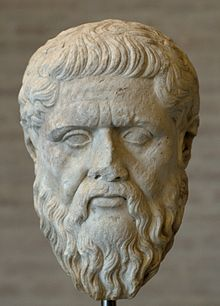
\includegraphics[width=0.3\textwidth]{Bilder/kap3/platon} 
	\caption{Römische Kopie eines griechischen Platonporträts\cite{WikiPL}  \label{portraitPlaton}}
\end{figure}

\subsection{Aristoteles}
Aristoteles (* 384 v. Chr. in Stagira (Griechenland) - † 322 v. Chr. in Chalkis) war Wissenschaftler, Biologe, Physiker und Philosoph. 

Als Sohn eines reiches Artzes war es ihm gegönt Platons Akademie zu besuchen. Er befasste sich zunächst mit mathematischen und dialekitschen Themen. Nach und nach begann er mit der Verfassung von eigenen Werken. Aristoteles blieb etwa 20 Jahre an der Akademie als Student und später als Lehrer. Nach dem Tod Platons verließ er Athen und seine sogenannten \glqq Reisejahre\grqq\ begannen. Während der Reisejahre ging Aristoteles auf Einladung von Philipp II. nach Mieza. Dort soll er den Sohn Alexander unterrichten. Dieser wird im Laufe der Geschichte zu Alexander der Große. Sein Weg führte ihn nun wieder nach Athen. Er forschte und lehrte an einem öffentlichen Gymnasium. Nachdem er sich von Alexander dem Großen und dem Königshaus abwandte, wurde ihm Gotteslästerung vorgeworfen. Daraufhin verließ er Athen und zog nach Chalkis. Dort starb er im Oktober 322 v. Chr.. 

Aristoteles zählt bis heute noch zu den bekanntesten und einflussreichsten Philosophen und Naturforschern. Zu den berühmtesten Werken des Aristoteles zählen seine Poetik, Politik und Metaphysik.
\footnote{vgl. \cite{Aristoteles1} und \cite{Aristoteles2}}
\begin{figure}[H]
\centering 
 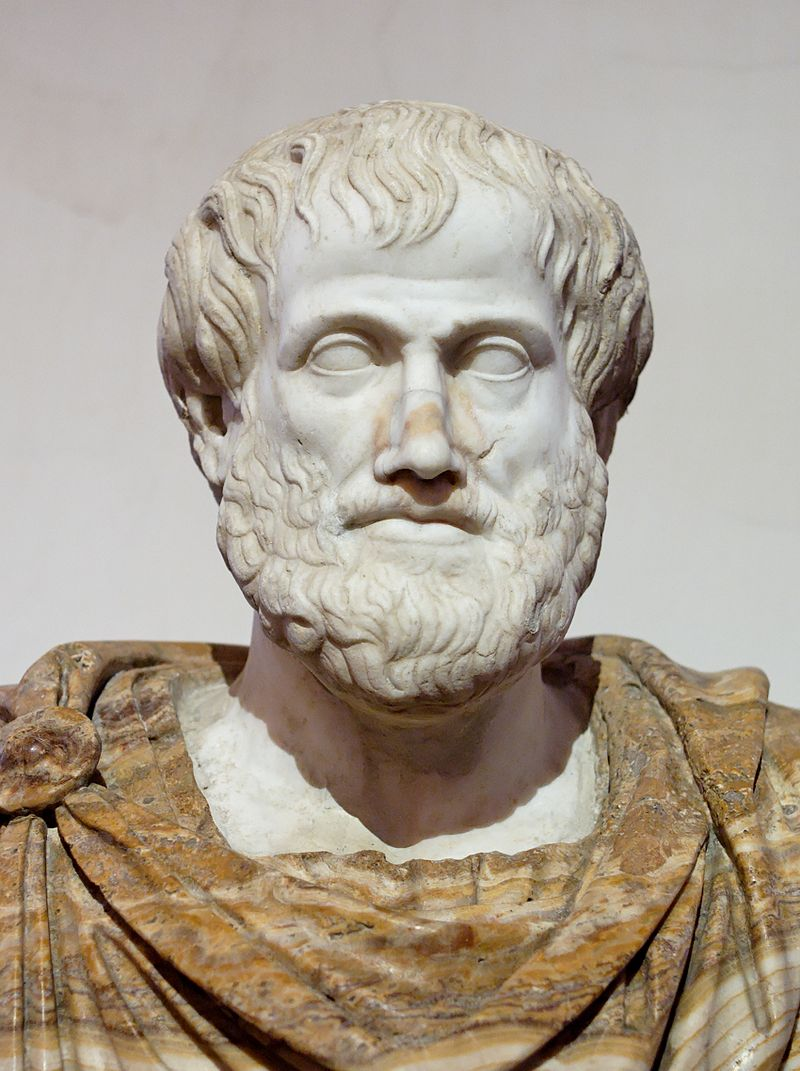
\includegraphics[width=0.3\textwidth]{Bilder/kap3/Aristoteles} 
 \caption{römische Kopie nach einer Skulptur des Bildhauers Lysippos \cite{WikiAR}  \label{portraitAristotles}}
\end{figure}

\subsection{Friedrich Nietzsche}
Friedrich Wilhelm Nietzsche (* 15. Oktober 1844 in Röcken - † 25. August 1900 in Weimar) war ein deutscher klassischer Philologe.

Bereits in seiner Jugendzeit fiel er durch überdurchschnittliche sprachliche sowie musikalische Fähigkeiten auf.
Während seines Studiums der klassischen Philologie sowie Theologie in Bonn und Leipzig beschäftigte er sich ausgiebig mit den Werken
\footnote{Maßgeblichen Einfluss auf ihn hatte Schopenhauers Hauptwerk \enquote{Die Welt als Wille und Vorstellung}. vgl. \cite{Schopenhauer1}}
des Philosophen Arthur Schopenhauers, die durch ihren Pessimismus seine Weltanschauung nachhaltig beeinflussten.
Des Weiteren übte auch Richard Wagner, Komponist und Freund Nietzsches, Einfluss auf sein Denken aus.

Nach dem Studium der klassischen Philologie sowie Theologie wurde er bereits im Alter von 25 Jahren zum Professor an die Universität Basel berufen.
Aufgrund körperlicher Beschwerden legte er nach 10 Jahren seine Professur nieder und widmete sich daraufhin weitestgehend von Mitmenschen isoliert vollkommen der Philosophie.
Weitere 10 Jahre vergingen bis sich sein körperlicher und psychischer Zustand soweit verschlechterte, dass er zu einem Pflegefall wurde und schlussendlich starb.

Durch seine philosophischen Schriften, darunter sein Hauptwerk \enquote{Also sprach Zarathustra}, erlangte Nietzsche postum Weltberühmtheit.\footnote{vgl. \cite{Nietzsche1}, \cite{Nietzsche2}, \cite{Nietzsche3} und \cite{Nietzsche4}}

\begin{figure}[H]
\centering 
 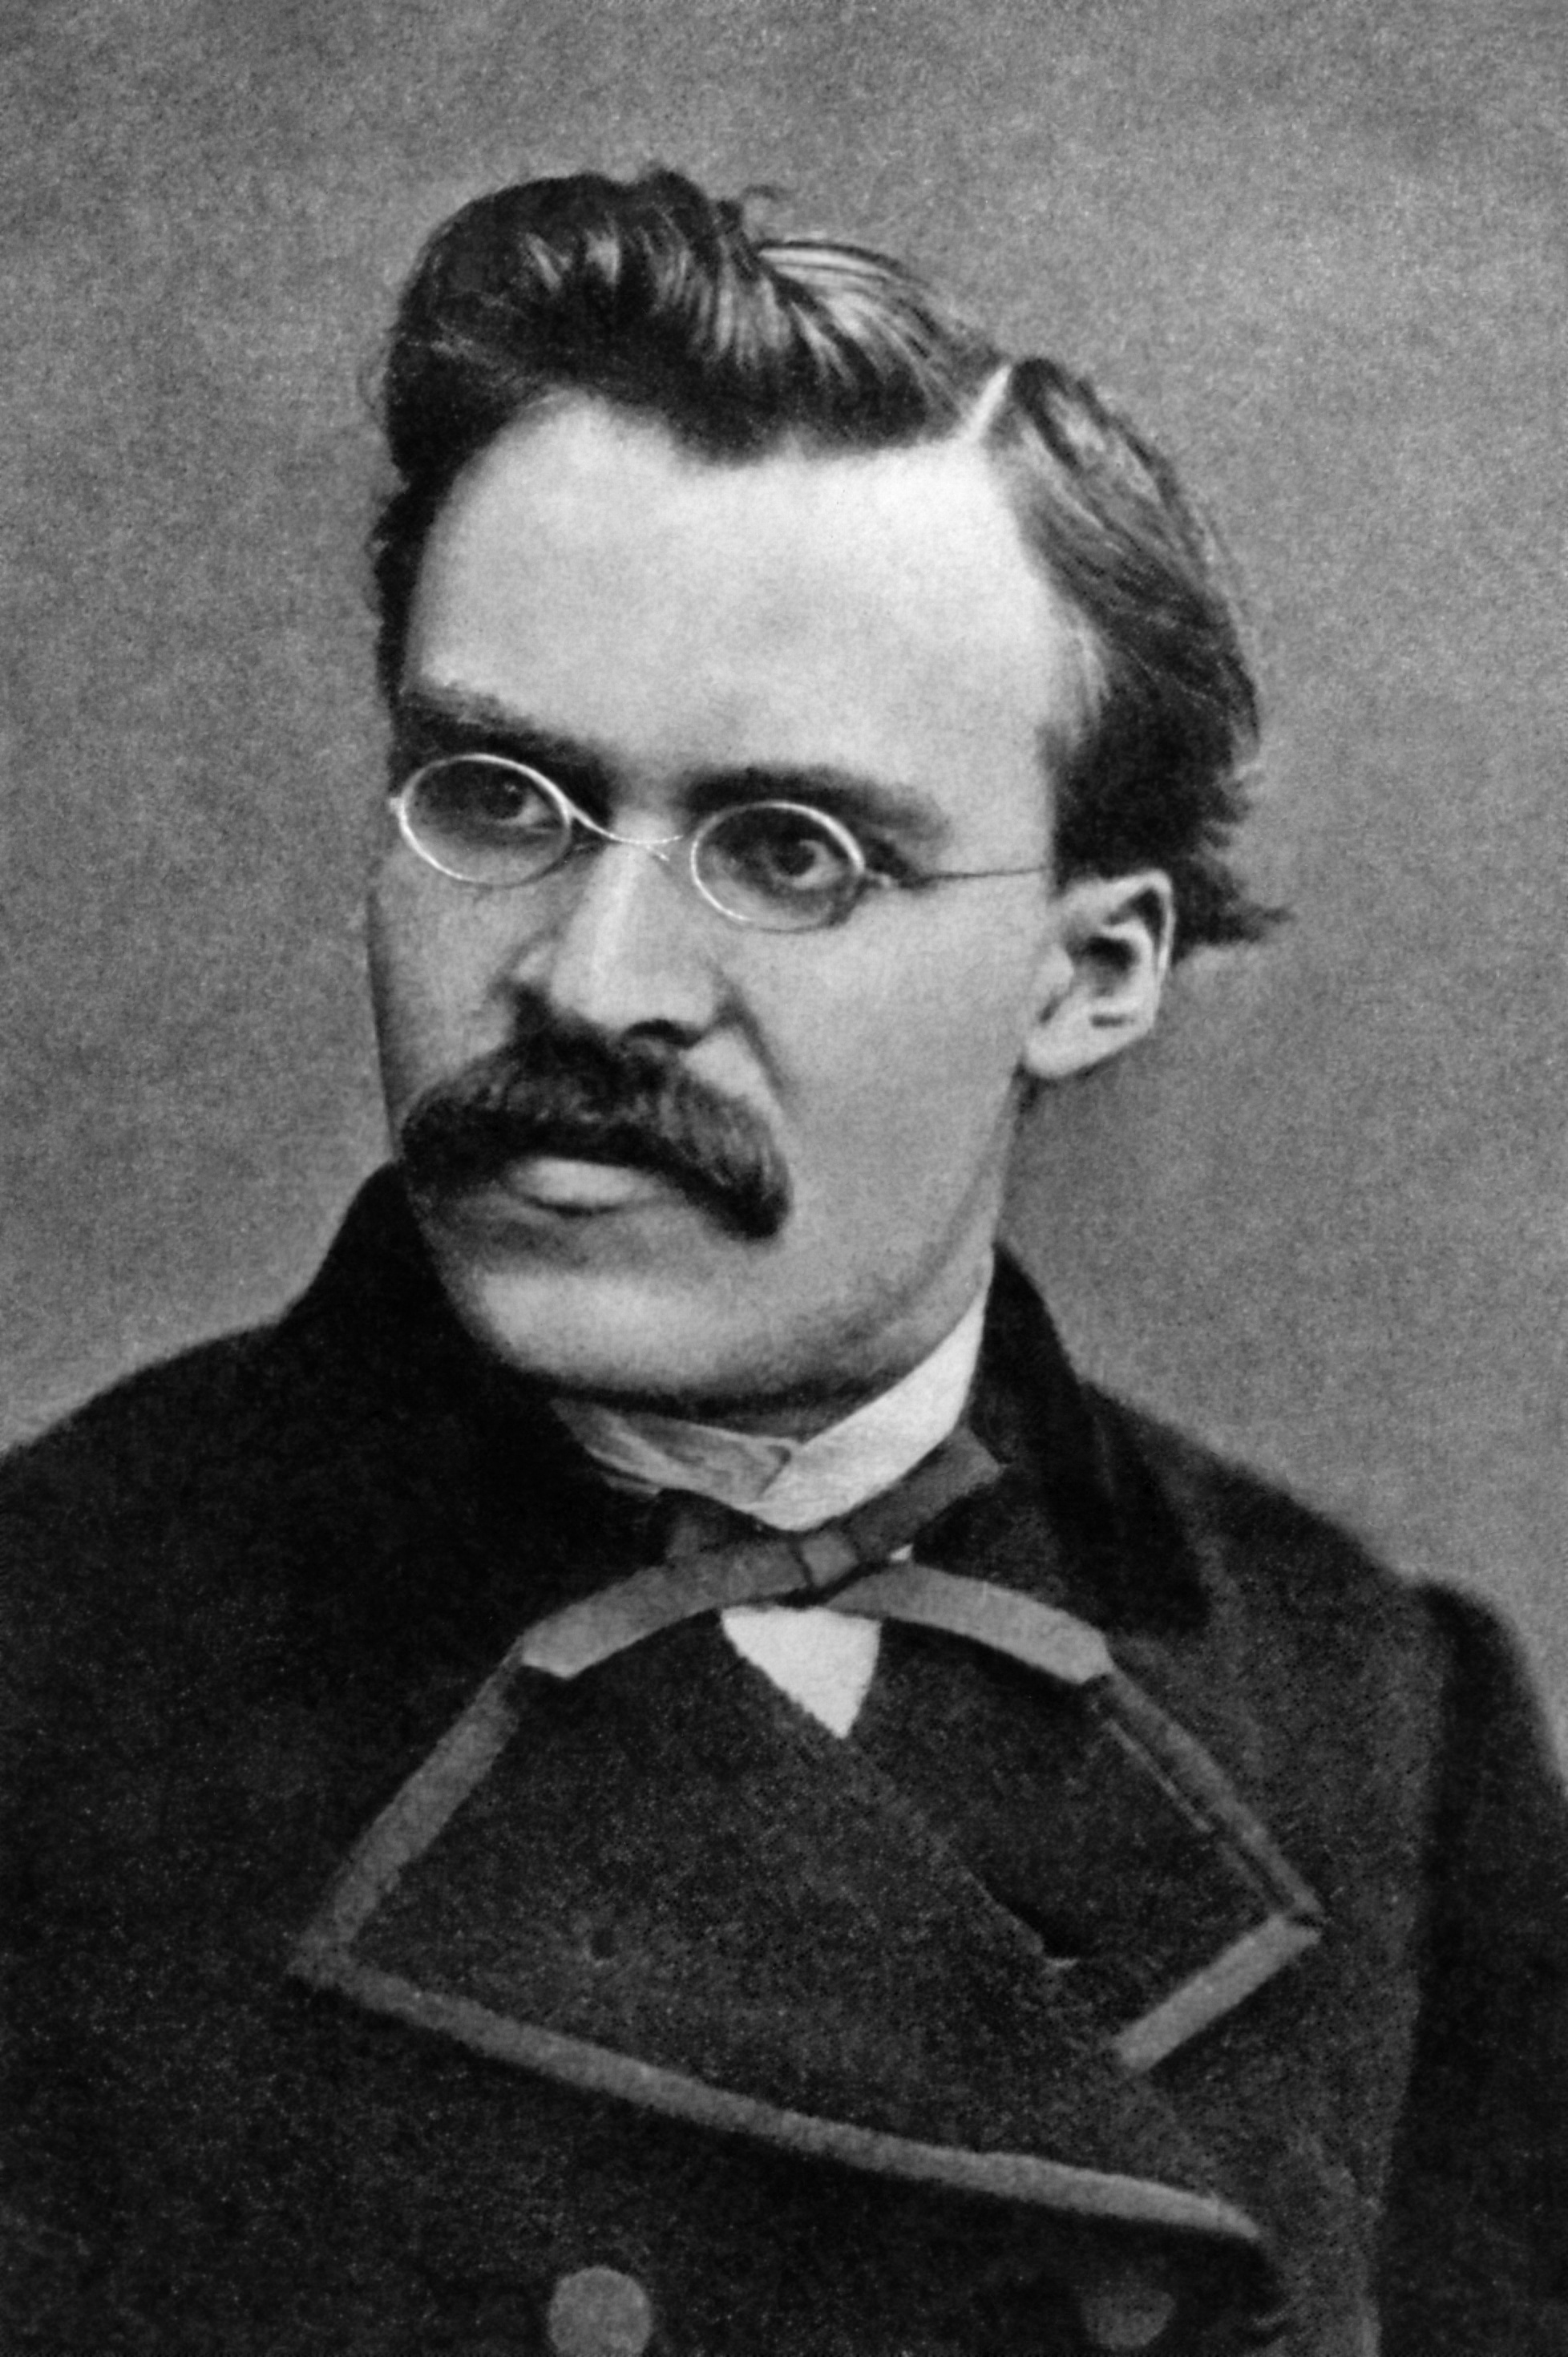
\includegraphics[width=0.3\textwidth]{Bilder/kap3/nietzschePortrait} 
 \caption{Friedrich Nietzsche um 1869.\cite{WQ14}  \label{portraitNietzsche}}
\end{figure}




